\subsubsection{\ac{drc}}\label{subsubsec:drc}

\citet{DRC_2020} propose a method called \ac{drc} 
that aims to address the issue of high intra-class diversities in existing deep clustering methods.
Even though the \ac{ap} can be similar for different samples, their \ac{af} can be different 
as illustrated in \autoref{fig:drc_af_ap}.
They claim that existing methods cluster dissimilar feature space representations \ac{af} together,
due to the usage of the maximum sensitivity of the softmax function used during cluster assignment.
\ac{drc} aims to address this issue by considering both the \ac{af} and the \ac{ap} during clustering.

\begin{figure}[h] % h = here, t = top, b = bottom, p = page of floats
    \centering
    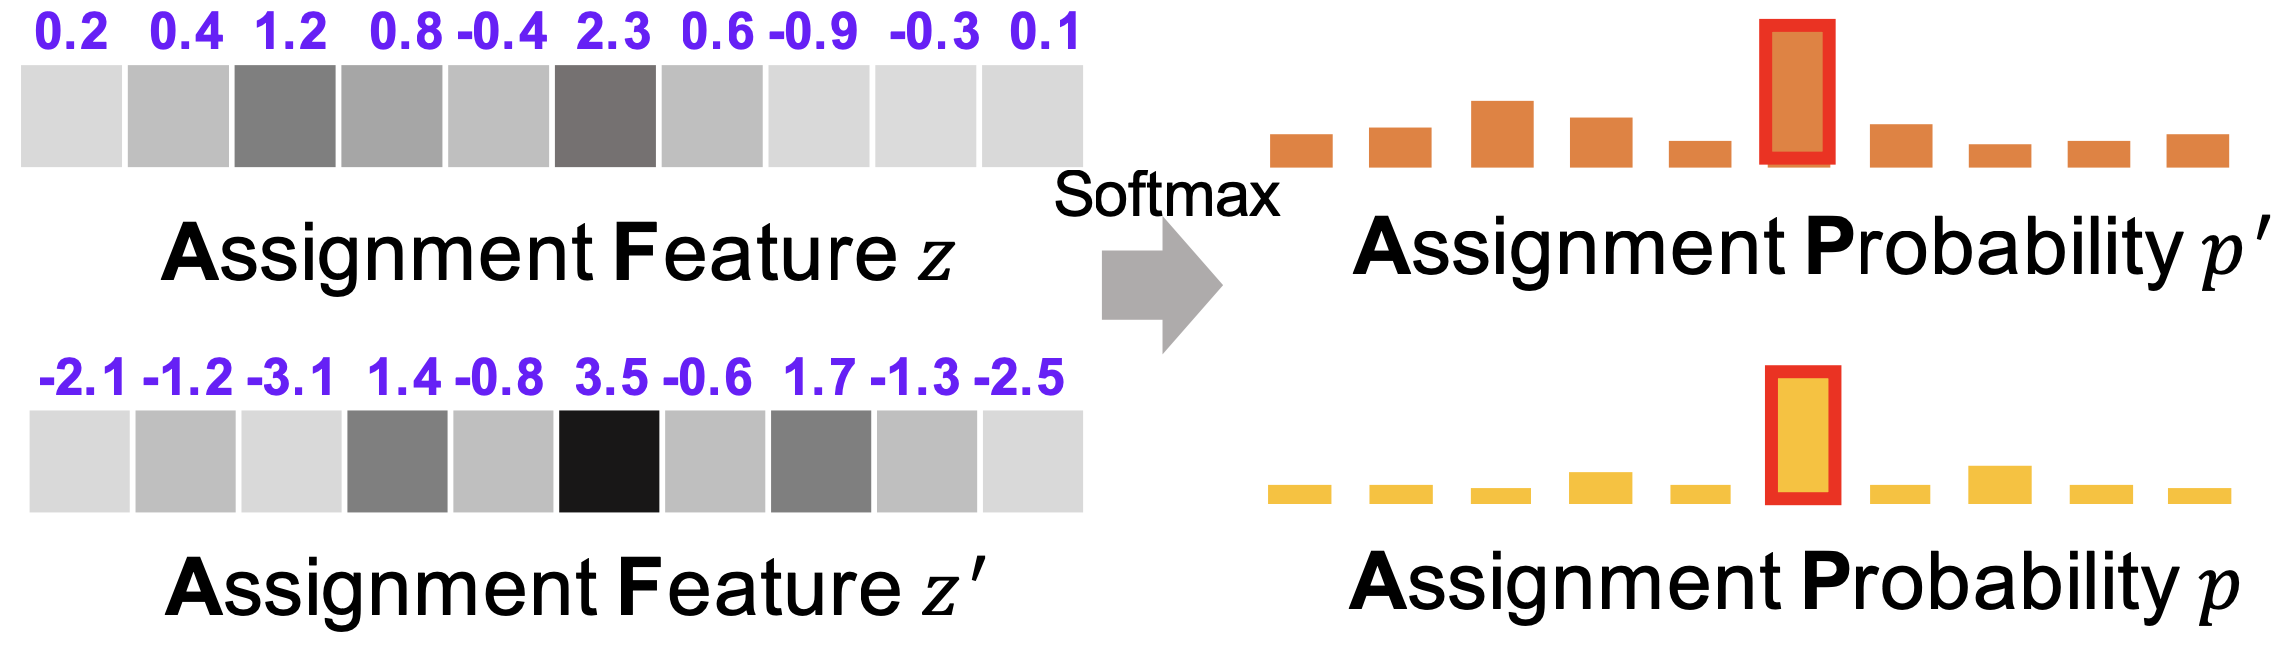
\includegraphics[width=300pt]{images/DRC_af_ap.png}
    \caption{Similar \ac{ap} values for different samples, but different \ac{af} values from \citet{DRC_2020}.
    Cluster assignment based on only \ac{ap} values can result in high intra-cluster diversities.}
    \label{fig:drc_af_ap}
\end{figure}

The \ac{af} $z_i$ are obtained from a \ac{cnn} with a fully connected layer, i.e. $z_i = f_\theta(x_i)$.
The \ac{ap} are obtained from the softmax function from \eqref{eq:ap}. 
Each sample $x_i$ is assigned to the cluster $j$ with the highest \ac{ap} value $p_{ij}$.
Optimally, the samples of a certain latent class should belong to the same cluster.

\begin{equation}
    p_{ij} = \frac{e^{z_{ij}}}{\sum_{K}^{t=1}e^{z_{it}}}, j \in \left[1,K\right]
    \label{eq:ap}
\end{equation}

\citeauthor{DRC_2020} present the loss function $\mathcal{L} = \mathcal{L}_{AF} + \mathcal{L}_{AP}  + \lambda \mathcal{L}_{CR}$  consisting of three terms.
The first term $\mathcal{L}_{AF}$ is the \ac{af} loss, which enforces similar representations of the sample and its positive transformation.
The second term $\mathcal{L}_{AP}$ is the \ac{ap} loss, which enforces the positive pairs of a sample and its augmentation 
to be assigned to the same cluster.
The third term $\mathcal{L}_{CR}$ is the cluster regularization loss, which penalizes clusterings where most samples are assigned to a minority of clusters.